\documentclass{article}
\usepackage{graphicx} % Required for inserting images
\usepackage{tabularx}
\usepackage{float}
\usepackage{longtable}
\usepackage[export]{adjustbox}

\title{Obliczenia Naukowe Lista 2}
\author{Bartłomiej Puchała}
\date{November 6, 2023}

\begin{document}

\maketitle

\section{Zadanie 1}
\subsection{Opis problemu}
Problem polega na powtórzeniu zadania 5 z listy 1, czyli obliczeniu iloczynu skalarnego dwóch wektorów, ale usunięciu ostatniej 9 z $x_4$ oraz ostatniej 7 z $x_5$.
\\
\subsection{Rozwiazanie}
\begin{verbatim}
function calc_forwards(T, vecX, vecY, n)
    sum = one(T) - 1
    for i in 1:n 
        sum += vecX[i] * vecY[i]
    end
    return sum
end

function calc_backwards(T, vecX, vecY, n)
    sum = one(T) - 1
    curr = n
    while curr >= 1
        sum += vecX[curr] * vecY[curr]
        if curr - 1 >= 1
            curr -= 1
        else
            break
        end
    end
    return sum
end
\end{verbatim}
\vspace{2em}

\begin{verbatim}
function calc_descending(T, vecX, vecY) 
    sum_positive = one(T) - 1
    sum_negative = one(T) - 1
    sum = one(T) - 1
    tmp_positive = T[]
    tmp_negative = T[]
    if length(vecX) == length(vecY)
        for (i, j) in zip(vecX, vecY)
            if i * j > 0
                push!(tmp_positive, i * j)
            else 
                push!(tmp_negative, i * j)
            end
        end
        sort!(tmp_positive, rev = true)
        sort!(tmp_negative)
        for i in tmp_positive
            sum_positive += i
        end 
        for j in tmp_negative 
            sum_negative += j
        end
        sum = sum_positive + sum_negative
    else
        println("Wektory nie są prawidłowe")
    end
end
\end{verbatim}
\begin{verbatim}
function calc_ascending(T, vecX, vecY)
    sum_positive = one(T) - 1
    sum_negative = one(T) - 1
    sum = one(T) - 1
    tmp_positive = T[]
    tmp_negative = T[]
    if length(vecX) == length(vecY)
        for (i, j) in zip(vecX, vecY)
            if i * j > 0
                push!(tmp_positive, i * j)
            else 
                push!(tmp_negative, i * j)
            end
        end
        sort!(tmp_positive)
        sort!(tmp_negative, rev = true)
        for i in tmp_positive
            sum_positive += i
        end 
        for j in tmp_negative
            sum_negative += j 
        end
        sum = sum_positive + sum_negative
    end
end
\end{verbatim}

\subsection{Wyniki oraz interpretacja}
\vspace{10pt}
\setlength{\tabcolsep}{2pt}
\renewcommand{\arraystretch}{1.4}
\begin{tabularx}{\linewidth}{|l|Y|X|}
\hline
Algorytm & Float32 & Roznica Float32 \\
\hline
W Przód & -0.4999443 & 0 \\
\hline
W Tył & -0.4543457 & 0 \\
\hline
Od Najw. & -0.5 & 0 \\
\hline
Od Najm. & -0.5 & 0 \\
\hline
\end{tabularx} \\
\vspace{25pt} \\
\setlength{\tabcolsep}{2pt}
\renewcommand{\arraystretch}{1.4}
\begin{tabularx}{\linewidth}{|l|Y|X|}
\hline
Algorytm & Float64 & Roznica Float64 \\
\hline
W Przód & -0.004296342739891585 & 0.004296342842410399 \\
\hline
W Tył & -0.004296342998713953 & 0.004296342842280865 \\
\hline
Od Najw. & -0.004296342842280865 & 0.004296342842280865 \\
\hline
Od Najm. & -0.004296342842280865 & 0.004296342842280865 \\
\hline
\end{tabularx} \\
\vspace{25pt} \\
Niewielkie zmiany w danych powodują różnice w otrzymywanych wynikach nawet o rząd wielkości $10^{-3}$.
\subsection{Wnioski}
Widząc problem, na którego wyniki znacząco wpływają nawet niewielkie zmiany w danych wejściowych sugeruje o złym poziomie uwarunkowania problemu.  
\vspace{20pt}
\section{Zadanie 2}
\subsection{Opis problemu}
Zadanie polega na narysowaniu wykresu funkcji 
$$f(x) = e^{x}\ln{(1 + e^{-x})}$$
w co najmniej dwóch programach do wizualizacji. Następnie należy policzyć granicę funkcji $\lim_{x \to \infty}f(x)$ i porównać wykres funkcji z obliczoną granicą.
\subsection{Rozwiazanie}

\begin{figure}[H] 
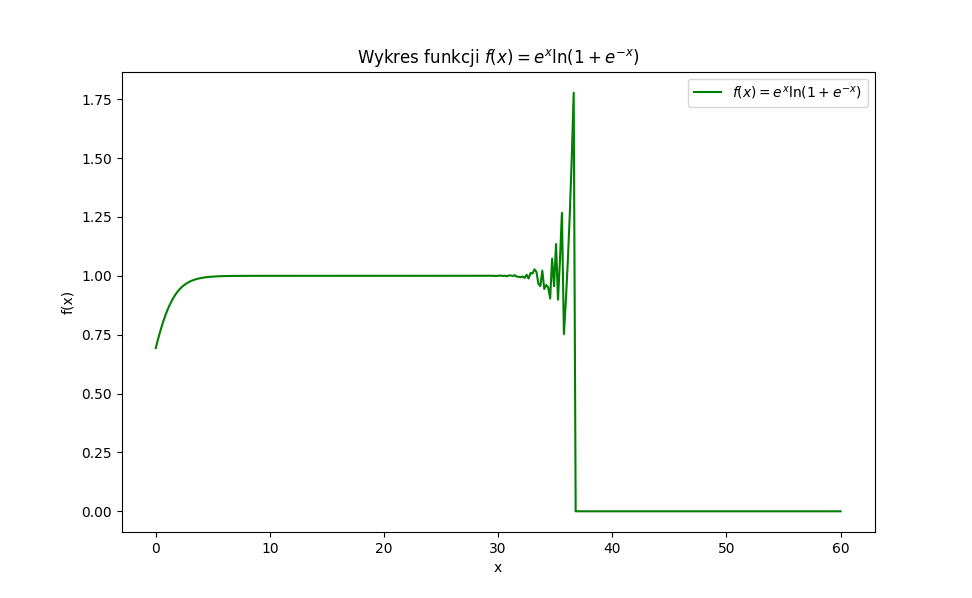
\includegraphics[width=0.95\textwidth, height=6.25cm,inner]{python_chart.png}
\caption{Wykres funkcji w Python(Matplotlib)}
\label{fig:figure_xx}
\end{figure}

\begin{figure}[H] 
\centering
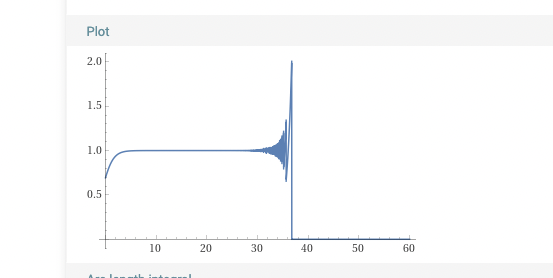
\includegraphics[width=0.95\textwidth, height=6.25cm,inner]{wolfr_ch.png}
\caption{Wykres funkcji w WolframAlpha}
\label{fig:figure_xxyy}
\end{figure}
\vspace{10pt}

$$\lim_{x \to \infty}e^{x}\ln{(1 + e^{-x})} = \lim_{x \to \infty}\frac{\ln{(1+e^{-x})}}{e^{-x}} = lim_{x \to \infty}\frac{-e^{-x}}{(1+e^{-x})*(-e^{-x})} = lim_{x \to \infty}\frac{1}{1 + e^{-x}} = 1 $$ 
Obliczona granica w nieskończoności przyjmuje wartość 1, granica została policzona przy pomocy metody de l’Hospitala.

\subsection{Wyniki i interpretacja}
Możemy zauważyć że wykres funkcji $f(x)$ w okolicach punktu $x=30$ staje się niestabilny a wartości zaczynają odbiegać od oczekiwanych. Następnie wartości zaczynają zbiegać do $0$, co jest sprzeczne z wynikiem obliczonej granicy $\lim_{x \to \infty}$.
\subsection{Wnioski}
Wartości zaczynają odbiegać od oczekiwanych dla $x$ w przedziale [30,40] z powodu faktu, że wartość $e^{-x}$ zbliża się do wartości epsilona maszynowego, więc wykres oscyluje wokół $1$, odbiega i zaczyna spadać do zera, co wynika z faktu, że wartość $\ln{(1 + e^{-x})}$ jest równa 0, bo wartość macheps została przekroczona.
\section{Zadanie 3}
\subsection{Opis problemu}
Zadanie polega na rozwiązaniu układu równań liniowych $$Ax=b$$ dla danej macierzy 
współczynników $A \in \mathbb{R}^{n \times n}$ i wektora prawych stron $b \in \mathb{R}^{n}$. Macierz $A$ ma być generowana jako macierz Hilberta($A=H_n$), gdzie n jest stopniem tej macierzy i jako ($A=R_n$), gdzie $R_n$ jest losową macierzą stopnia n z zadanym wskaźnikiem uwarunkowania $c$. Ten układ równań należy rozwiązać za pomocą $2$ algorytmów, algorytmu eliminacji Gaussa($x=A\div{b}$) oraz dla algorytmu($x=inv(A)*b$).
\subsection{Rozwiazanie}
\begin{verbatim}
function calculate_relative_error(x, reference_x)
    # Norma Euklidesowa roznicy wektorów
    error_norm = norm(x - reference_x) 
    # norma Euklidesowa wektora referencyjnego
    reference_norm = norm(reference_x)
    # Bląd względny
    relative_error = error_norm / reference_norm
    return relative_error
end

function calcGauss(A, b) 
    x = A \ b
    return x
end
function calcInverse(A, b)
    x = inv(A) * b
    return x
end

# Funkcja do generowania macierzy Hilberta
function hilb(n::Int64)
    H = zeros(Float64, n, n)
    for i in 1:n 
        for j in 1:n
            H[i, j] = 1 / (i + j - 1)
        end
    end
    return H
end

# Funkcja do generowania macierzy danego rozmiaru i na podstawie podanego uwarunkowania
function matcond(n::Int, c::Float64)
    if(n < 2)
        return "Size of n should be > 1"
    end
    A = rand(n, n)
    F = svd(A) # rozkład svd(wedlug wartości osobliwych)
    U, S, V = F # U to macierz lewych wektorów osobliwych
    #S to macierz diagonalna wartości osobliwych, V to macierz prawych wektorów osobliwych
    return U * diagm(0 => [LinRange(1.0, c, n);])*V # pomnozenie macierzy U i V^T, 
    # gdzie V^T to macierz transponowana przez macierz diagonalną S z odpowiednimi 
    # wartościami na diagonali jako zakres od 1.0 do c z równymi odstępami
end
\end{verbatim}
\subsection{Wyniki oraz interpretacja}
\begin{enumerate}
    \item Wyniki dla Macierzy Hilberta($H_n$)
    
\setlength{\tabcolsep}{2pt}
\renewcommand{\arraystretch}{1.6}
\newcolumntype{Y}{>{\raggedright\arraybackslash}X}
\begin{tabularx}{\textwidth}{|l|Y|Y|Y|}
\hline
n & Gauss Error & Inverse Error & Condition \\
\hline
2 & 7.021666937153401e-16 & 0.0 & 19.281470067903967 \\
\hline
3 & 2.7375497437671545e-15 & 2.329670154318109e-14 & 524.0567775860627 \\
\hline
4 & 2.163452954752009e-13 &  3.4135644425146874e-13 & 15513.738738929662 \\
\hline
5 & 2.7871931343743106e-13 & 7.455637944774642e-12 & 476607.2502419222 \\
\hline
6 & 3.347582158492704e-10 & 1.2827865807782325e-10 & 1.4951058641931808e7 \\
\hline
7 & 1.0714660570624442e-8 & 1.1527300819247877e-8 & 4.7536735651983196e8 \\
\hline
8 & 4.415963229892491e-7 & 3.79672835736301e-7 & 1.5257576052786306e10 \\
\hline
9 & 1.1753313049338465e-5 & 1.4840163876939037e-5 & 4.931539099297127e11 \\
\hline
10 & 0.00022069259050910798 & 0.0003816537448426628 & 1.602489743907797e13 \\
\hline
11 & 0.0061370127224061755 & 0.005027508456077255 & 5.219592223385588e14 \\
\hline
13 & 1.9340328542478238 & 2.176661432102452 & 6.738714767183357e17 \\
\hline
15 & 14.530780684593466 & 12.429282151240843 & 2.3228053763031325e17 \\
\hline
17 & 5.702847199359304 & 7.400447213245778 & 6.968485027955343e17 \\
\hline
19 & 7.977164583041656 & 12.28072952372789 & 1.777632773409892e18 \\
\hline
21 & 43.504485883896244 & 154.96073707047393 & 4.834811654527856e18 \\
\hline
23 & 21.634056047548167 & 34.13604551118164 & 1.1344683590683766e18 \\
\hline
25 & 23.572600504144535 & 21.490537874421143 & 2.0216257487362834e19 \\
\hline
27 & 30.11002787196579 & 72.14426727588254 & 2.766053659397318e18 \\
\hline
29 & 18.47553583161393 & 19.28944178353934 & 2.6372941826255836e18 \\
\hline
\end{tabularx} \\
\vspace{25pt} \\
Jak widać macierz Hilberta jest przykładem macierzy źle uwarunkowanej, zatem numerycznie rozwiązywanie nawet niewielkich układów równań z tą macierzą jest praktycznie niemożliwe. Można to zauważyć po szybko wzrastającym wskaźniku uwarunkowania($cond(x)$), który dla macierzy 10 x 10 osiąga rząd wielkości $10^{13}$.
\newpage
\item Wyniki dla Macierzy Losowej($R_n$)
\end{enumerate}
\vspace{25pt}

\setlength{\tabcolsep}{2pt}
\renewcommand{\arraystretch}{1.4}
\begin{tabularx}{\textwidth}{|l|Y|Y|X|}
\hline
n & Cond & Gaus Error & Inverse error \\
\hline
5 & 1.0 & 2.164223099578636e-16 & 2.6737711109153337e-16 \\
\hline
5 & 10.0 & 4.2130001622920406e-16 & 4.2130001622920406e-16 \\
\hline
5 & 1000.0 & 1.4325319156034877e-14 & 2.470998322584863e-14 \\
\hline
5 & 1.0e7 & 1.3871114407994677e-10 & 2.598008332320691e-10 \\
\hline
5 & 1.0e12 & 5.733757560742947e-5 & 4.962195967762327e-5 \\
\hline
5 & 1.0e16 & 0.01175107665021737 & 0.0642202714205108 \\
\hline
10 & 1.0 & 3.940900794429957e-16 & 2.0770370905276122e-16 \\
\hline
10 & 10.0 & 3.3306690738754696e-16 & 2.531698018113677e-16 \\
\hline
10 & 1000.0 & 8.056119772367459e-15 & 3.39093083129075e-14 \\
\hline
10 & 1.0e7 & 2.376733646052788e-10 & 4.706835956915451e-10 \\
\hline
10 & 1.0e12 & 3.203285562720351e-5 & 5.190000397273812e-5 \\
\hline
10 & 1.0e16 & 0.110173622460718 & 0.11403535478679437 \\
\hline
20 & 1.0 & 6.951095629092364e-16 & 5.063396036227354e-16 \\
\hline
20 & 10.0 & 1.0987843116542347e-15 & 1.0755419851390038e-15 \\
\hline
20 & 1000.0 & 6.581303858479593e-14 & 5.205047726233623e-14 \\
\hline
20 & 1.0e7 & 5.5720873743889447e-11 & 2.321665025423311e-10 \\
\hline
20 & 1.0e12 & 6.6992662457360325e-6 & 1.7828796469037173e-5 \\
\hline
20 & 1.0e16 & 0.2970415720198951 & 0.6241706046197695 \\
\hline
\end{tabularx} \\
\vspace{18pt} \\
\subsection{Wnioski}
Uwarunkowanie macierzy Hilberta ma bezpośredni wpływ na to, że wraz ze wzrostem $n$ błędy się zwiększają przy dowolnej metodzie wraz z coraz większym $cond(x)$. Dlatego wskaźnik uwarunkowania jest ważnym narzędziem w analizie numerycznej i pomaga określić, czy dana macierz jest odpowiednia do konkretnych obliczeń.

\section{Zadanie 4}
\subsection{Opis problemu}
Zadanie polega na sprawdzeniu obliczonych pierwiastków $z_k$  $1 \leq k \leq 20$ wielomianu Wilkinsona, obliczeniu $\left|P(z_k)\right|$, $\left|p(z_k)\right|$, i $\left|z_k - k\right|$. Należy również powtórzyć eksperyment Wilkinsona ze zmienionym współczynnikiem.
\subsection{Rozwiązanie}
\begin{verbatim}
function p(x) 
    val = one(Float64)
    for i in 20:-1:1
        val = val * (x - i)
    end
    return val
end

coefficients = [1, -210.0-2.0^(-23), 20615.0,-1256850.0,
      53327946.0,-1672280820.0, 40171771630.0, -756111184500.0,          
      11310276995381.0, -135585182899530.0,
      1307535010540395.0,     -10142299865511450.0,
      63030812099294896.0,     -311333643161390640.0,
      1206647803780373360.0,     -3599979517947607200.0,
      8037811822645051776.0,      -12870931245150988800.0,
      13803759753640704000.0,      -8752948036761600000.0,
      2432902008176640000.0]

P = Polynomial(reverse(coefficients))
println(P)

roots = Polynomials.roots(P)
println(roots)


for k in 1:20
    println("$k & $(abs(P(roots[k]))) & $(abs(p(roots[k]))) & $(abs(roots[k] - k))")
end
\end{verbatim}
\subsection{Wyniki i interpretacja}
\vspace{10pt}
\setlength{\tabcolsep}{2pt}
\renewcommand{\arraystretch}{1.4}
\begin{tabularx}{\textwidth}{|l|Y|Y|X|}
\hline
k & $|P(z_k)|$ & $|p(z_k)|$ & $|z_k - k|$ \\
\hline
1 & 1603.9573920179469 & 304572.04260797694 & 1.6653345369377348e-14 \\
\hline
2 & 7032.126244053075 & 7.378697629496515e19 & 8.602007994795713e-13 \\
\hline
3 & 363020.53660426877 & 3.320413934571126e20 & 3.3646685437815904e-10 \\
\hline
4 & 4.1297007568024816e6 & 8.854436933250461e20 & 3.0104239989725556e-8 \\
\hline
5 & 3.075695036659063e7 & 1.844675459361676e21 & 8.773618791479976e-7 \\
\hline
6 & 1.4257935012621844e8 & 3.3203908470754844e21 & 1.3036540314814715e-5 \\
\hline
7 & 5.24632388586803e8 & 5.423631524959937e21 & 0.00011769796309923919 \\
\hline
8 & 1.7358866242071867e9 & 8.261841653520567e21 &  0.0007083981118194416 \\
\hline
9 & 5.1002248626897955e9 & 1.1966108418294833e22 & 0.003039097772564503 \\
\hline
10 & 1.166611991635824e10 & 1.655343433307367e22 & 0.009425364817383652 \\
\hline
11 & 3.127208130563727e10 & 2.246553909518422e22 & 0.02299817354506395 \\
\hline
12 & 6.1418141120587135e10 & 2.89153886820604e22 & 0.040566592069646745 \\
\hline
13 & 1.5300549815452048e11 & 3.7940459609615415e22 & 0.05950452401079254 \\
\hline
14 & 3.0985557081238544e11 & 4.633597782215305e22 & 0.06480991092200128 \\
\hline
15 & 5.010255098229966e11 & 5.875191008208141e22 & 0.05398301833971253 \\
\hline
16 & 9.394123675655612e11 & 7.034662578633065e22 & 0.03609096183973115 \\
\hline
17 & 2.3971581253245e12 & 8.555214312879987e22 & 0.0165393639009217 \\
\hline
18 & 5.670957056381105e12 & 1.0150796567230493e23 & 0.005602369314754441 \\
\hline
19 & 7.741019369389632e12 & 1.1988901833144277e23 & 0.0011451039164107613 \\
\hline
20 & 1.2178388919649346e13 & 1.4019287561968973e23 & 0.00011119342792653697 \\
\hline
\end{tabularx} \\
\vspace{10pt} \\
\begin{center}
    Wyniki dla wielomianu Wilkinsona
\end{center}
Można zauważyć, że wyniki otrzymywane dla kolejnych $k$, które są rozwiązaniami wielomianu w zbiorze liczb rzeczywistych($\mathbb{R}$) są coraz bardziej niedokładne, różnice między wartością otrzymywaną z $P(z_k)$ a $p(z_k)$ wynika z powodu róznych działań arytmetycznych.

\vspace{15pt}
\setlength{\tabcolsep}{2pt}
\renewcommand{\arraystretch}{1.4}
\begin{tabularx}{\textwidth}{|l|Y|Y|X|}
\hline
k & $|P(z_k)|$ & $|p(z_k)|$ & $|z_k - k|$ \\
\hline
1 & 10130.71275321466 & 9426.712753211954 & 7.749356711883593e-14 \\
\hline
2 & 56308.28771988236 & 53114.287721025175 & 8.29603052920902e-12 \\
\hline
3 & 807092.163108728 & 633550.7888912051 & 8.906004822506475e-10 \\
\hline
4 & 8.084860855411538e6 & 7.048149034054348e6 & 5.614410936161107e-8 \\
\hline
5 & 3.879198510577002e7 & 3.410921815648757e7 & 1.0868296920207854e-6 \\
\hline
6 & 1.4732257627258718e8 & 5.432787182756067e7 & 5.193150526494605e-6 \\
\hline
7 & 4.1411759028405327e8 & 1.0237654561324999e9 & 0.0002283049351108346 \\
\hline
8 & 5.02184047848722e8 & 1.6791947081836334e10 & 0.006980931819212444 \\
\hline
9 & 1.2260299344962182e9 & 1.3433655504423593e11 & 0.08227581314042176 \\
\hline
10 & 1.711412152637466e9 & 1.4837248370635044e12 & 0.6505270479399019 \\
\hline
11 & 1.711412152637466e9 & 1.4837248370635044e12 & 1.1105047852610384 \\
\hline
12 & 1.922343284948516e10 & 3.2968824832136562e13 & 1.665389446835571 \\
\hline
13 & 1.922343284948516e10 & 3.2968824832136562e13 & 2.0460081179778995 \\
\hline
14 & 2.78104055609644e11 & 9.547439978559046e14 & 2.518885830105916 \\
\hline
15 & 2.78104055609644e11 & 9.547439978559046e14 & 2.712916579182928 \\
\hline
16 & 1.0504983293359739e12 & 2.742163099611119e16 & 2.9060058491454366 \\
\hline
17 & 1.0504983293359739e12 & 2.742163099611119e16 & 2.8254814771679904 \\
\hline
18 & 6.884949792026641e12 & 4.252467839147873e17 & 2.454019284846941 \\
\hline
19 & 6.884949792026641e12 & 4.252467839147873e17 & 2.004325976483215 \\
\hline
20 & 9.72908249032009e11 & 1.3743636608789734e18 & 0.8469082068719089 \\
\hline
\end{tabularx}
\begin{center}
    Wyniki dla zmodyfikowanego wielomianu Wilkinsona
\end{center}
Po zaburzeniu współczynnika $-210$ przy $x^{19}$ o wartość $-2^{-23}$ rozwiązaniami wielomianu stają się pierwiastki zespolone. Przykładowo dla $k=19$ rozwiązaniem jest $19.50244401519765 + 1.9403279701116138im$. 
\subsection{Wnioski}
Wyznaczanie pierwiastków wielomianu Wilkinsona jest zadaniem źle uwarunkowanym, wynika to z faktu, że po zmianie współczynnika $a_{19}$ z $-210$ na $-210-2^{-23}$ powoduje duże zmiany w otrzymywanych wynikach. Wynika to z tego faktu:
$$h \approx \epsilon*\frac{z(r)}{\(w'(r)\)} $$ \\

gdzie r jest pierwiastkiem, $\epsilon$ jest precyzją arytmetyki, funkcja $z(r)$ jest zaburzeniem pierwiastka, a $w'(r)$ jest pochodną wielomianu. Natomiast niedokładności w obliczaniu zer wielomianu wynikały z faktu, że brakowało cyfr znaczacych do zapisu takich dużych współczynników w danej arytmetyce.
\vspace{20pt}

\section{Zadanie 5}
\subsection{Opis problemu}
Zadanie polega na przeprowadzeniu eksperymentów dla podanego równania rekurencyjnego:
$$p_{n+1} = p_n + rp_n(1-p_n)$$
\begin{enumerate}
    \item Wykonanie 40 iteracji wyrażenia dla danych $p_0 = 0.01$ i $r = 3$ w arytmetyce Float32
    \item Wykonanie 10 iteracji, zatrzymanie się, zastosowanie obcięcia wyniku i kontynuowanie dalej obliczenia w arytmetyce Float32
    \item Dla danych $p_0 = 0.01$ i $r = 3$ wykonanie 40 iteracji wyrażenia w arytmetyce Float32 i Float64
\end{enumerate}
\subsection{Rozwiazanie}
\begin{verbatim}
function calc_population(p::Float32, r::Float32, i::Float32)
    next_p::Float32 = one(Float32) - 1
    if i == 41
        return
    end
    next_p = p + r * p * (1 - p)
    println("$i & $next_p")
    return calc_population(next_p, r, i + 1)
end

p0 = Float32(0.01)
r = Float32(3.0)
i = Float32(1.0)
calc_population(p0, r, i)
\end{verbatim}
\subsection{Wyniki i interpretacja}
\begin{enumerate}
    \item Dla $40$ iteracji wyrażenia w arytmetyce Float32
    $$ x = p_{40} = 0.25860548$$

    \item Dla $40$ iteracji wyrażenia po zatrzymaniu i zastosowania obcięcia po 10 iteracji w arytmetyce Float32
    $$ x = p_{40} = 1.093568$$ \\

    \item Dla $40$ iteracji wyrażenia w arytmetyce Float64
    $$ x = p_{40} = 0.011611238029748606$$ \\
    Można zauważyć, że precyzja arymetyki jak i obcinanie cyfr znaczących jak w przypadku $1$ może mieć znaczący wpływ na otrzymywane wyniki.
\end{enumerate}
\subsection{Wnioski}
Aby odpowiednio rozwiązać równanie rekurencyjne w obliczeniach numerycznych, należy zwrócić uwagę na precyzję arytmetyki oraz na to, aby nie obcinać cyfr znaczących.

\section{Zadanie 6}
\subsection{Opis problemu}
Zadanie polega na przeprowadzeniu eksperymentów dla poniższego równania rekurencyjnego:
$$ x_{n+1} = x^{2}_n + c $$ \\
gdzie $n = 0,1,...$ i c jest pewną stałą. Należy przeprowadzić następujące eksperymenty:
\begin{enumerate}
    \item $c =-2$ i $x_0 = 1$
    \item $c =-2$ i $x_0 = 2$
    \item $c =-2$ i $x_0 = 1.99999999999999$
    \item $c =-1$ i $x_0 = 1$
    \item $c =-1$ i $x_0 = -1$
    \item $c =-1$ i $x_0 = 0.75$
    \item $c =-1$ i $x_0 = 0.25$
\end{enumerate}
\subsection{Rozwiazanie}
\begin{verbatim}
function calc_equation(x, c, i)
    if i == 41
        return
    end
    next_x = x^2 + c
    println("$i & $next_x")
    return calc_equation(next_x, c, i + 1)
end

c = -1.0
x_0 = 0.25
i = 1.0
calc_equation(x_0, c, i)
\end{verbatim}
\subsection{Wyniki oraz interpretacja}
\begin{enumerate}
    \item $c =-2$ i $x_0 = 1$ $\rightarrow$ $x = -1.0$
    \item $c =-2$ i $x_0 = 2$ $\rightarrow$ $x = 2.0$
    \item $c =-2$ i $x_0 = 1.99999999999999$ $\rightarrow$ $x = -0.3289791230026702$
    \item $c =-1$ i $x_0 = 1$ $\rightarrow$ $x = -1.0$
    \item $c =-1$ i $x_0 = -1$ $\rightarrow$ $x = -1.0$
    \item $c =-1$ i $x_0 = 0.75$ $\rightarrow$ $x = -1.0$
    \item $c =-1$ i $x_0 = 0.25$ $\rightarrow$ $x = 0.0$
\end{enumerate}
Przeprowadziłem iterację graficzną w WolframAlpha dla zadanych danych:

\begin{figure}[H] 
\centering
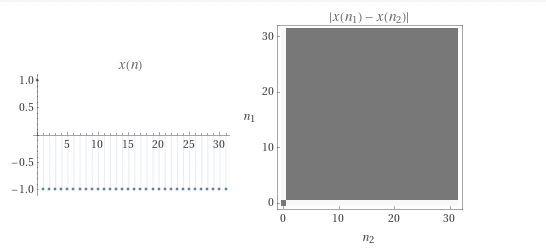
\includegraphics[width=0.85\textwidth, height=5cm]{6a.png}
\caption{$c = -2$, $x_0 = 1$}
\label{Fig_}
\end{figure}

\begin{figure}[H] 
\centering
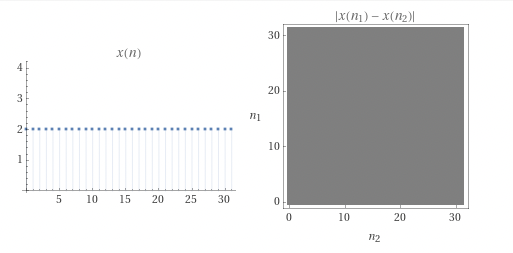
\includegraphics[width=0.85\textwidth, height=4.75cm]{6b.png}
\caption{$c = -2$, $x_0 = 2$}
\end{figure}

\begin{figure}[H] 
\centering
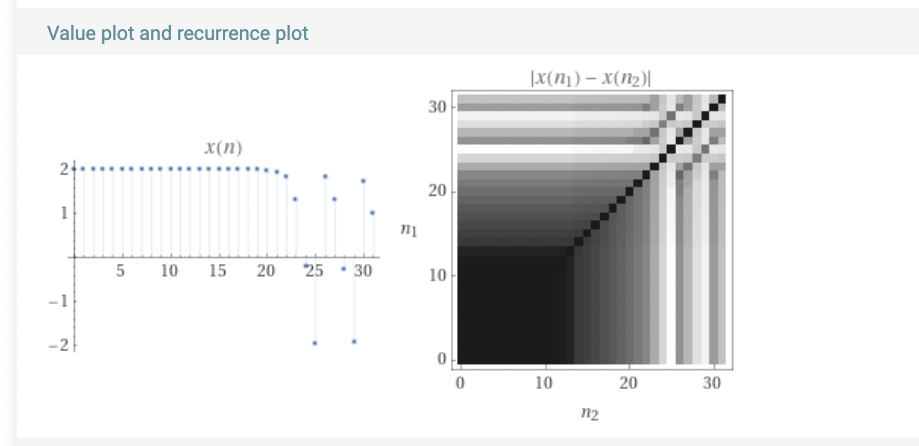
\includegraphics[width=0.9\textwidth, height=4.5cm]{6c.png}
\caption{$c = -2$, $x_0 = 1.99999999999999$}
\end{figure}

\begin{figure}[H] 
\centering
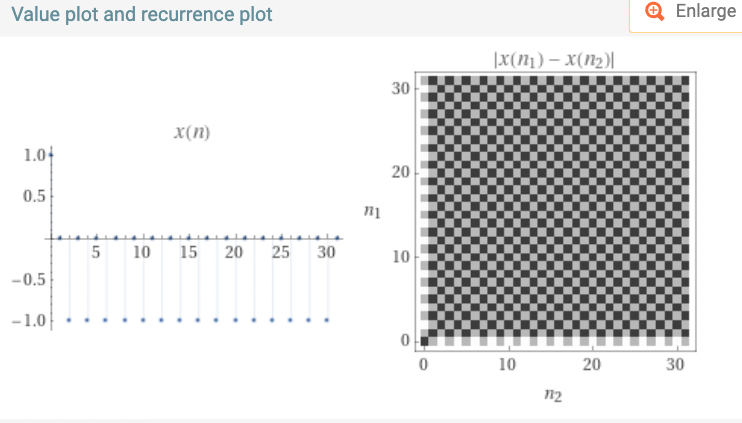
\includegraphics[width=0.85\textwidth, height=4.25cm]{6d.png}
\caption{$c = -1$, $x_0 = 1$}
\end{figure}

\begin{figure}[H] 
\centering
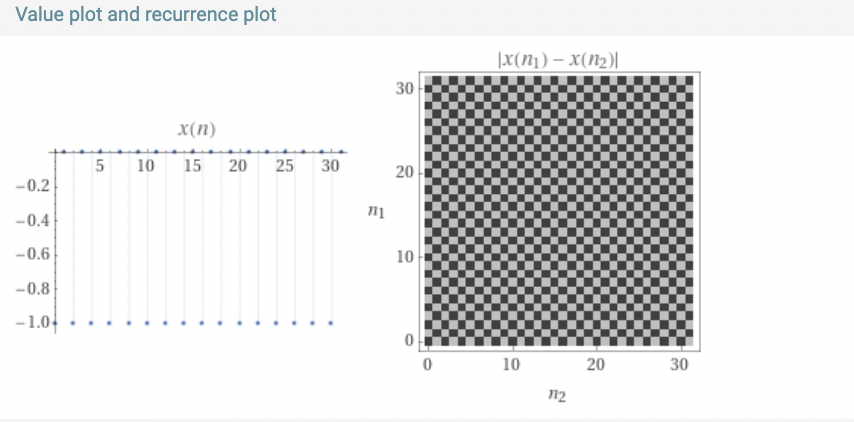
\includegraphics[width=0.9\textwidth, height=4.5cm]{6e.png}
\caption{$c = -1$, $x_0 = -1$}
\end{figure}

\begin{figure}[H] 
\centering
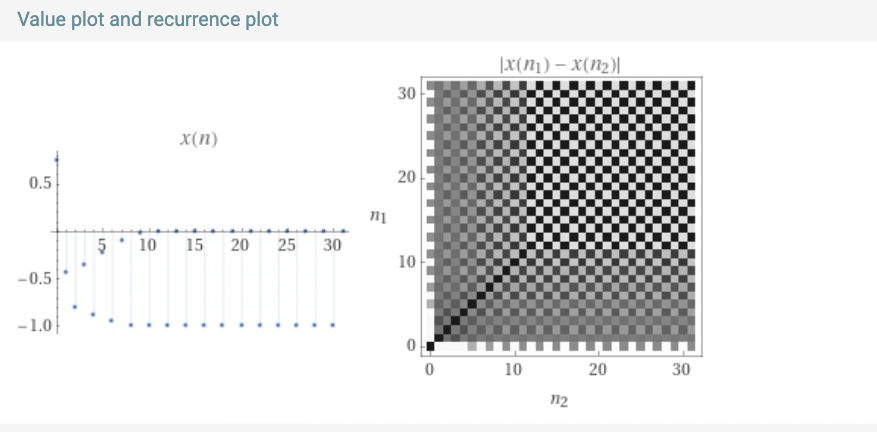
\includegraphics[width=0.9\textwidth, height=4.5cm]{6f.png}
\caption{$c = -1$, $x_0 = 0.75$}
\end{figure}

\begin{figure}[H] 
\centering
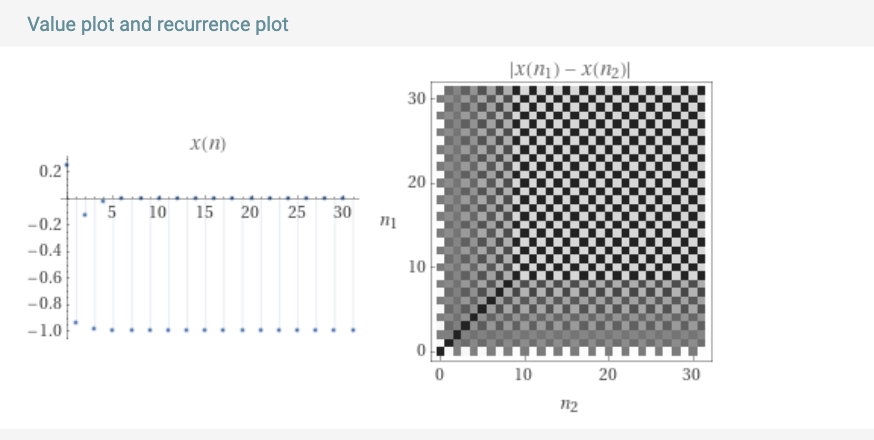
\includegraphics[width=0.9\textwidth, height=4.5cm]{6_last.png}
\caption{$c = -1$, $x_0 = 0.25$}
\end{figure}

\subsection{Interpretacja i Wnioski}
Wnioskiem z graficznych reprezentacji jest fakt, że w przypadku równań rekurencyjnych możemy uzyskać różną numeryczną stabilność dla różnych danych. Dla poniższych eksperymentów można zauważyć, że dla $x_0 = 1.99999999999999$ i $c = -2$ otrzymujemy niestabilne wyznaczanie kolejnych wyrazów ciągu, dla ($c=-1$ $x_0=0.25$ i $x_0=0.75$) otrzymujemy stabilizujace wyznaczanie, a dla danych ($x_0=1$ i dla $c=-2$ i $c=-1$) otrzymujemy całkowicie stabilne wyznaczanie. Warto również zwrócić uwagę, że wartość paraemtru np. $x_0$ wpływa na szybkość stabilizacji wyznaczania kolejnych wyrazów, widać to w przypadku ($c=-1$ $x_0=0.25$ i $x_0=0.75$), gdzie dla $x_0=0.25$ wyznaczanie wyrazów stablizuje się szybciej niż dla $x_0=0.75$. Dlatego odpowiednie dobieranie parametrów jest kluczowe do uzyskania stabilności i wiarygodnych wyników w analizie numerycznej.
\end{document}
